\begin{center}
	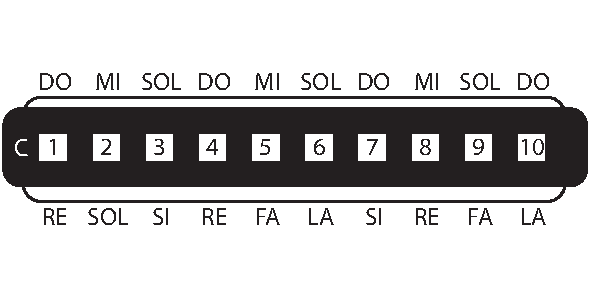
\includegraphics[width=10cm]{chapters/Note-Armonica.pdf}
	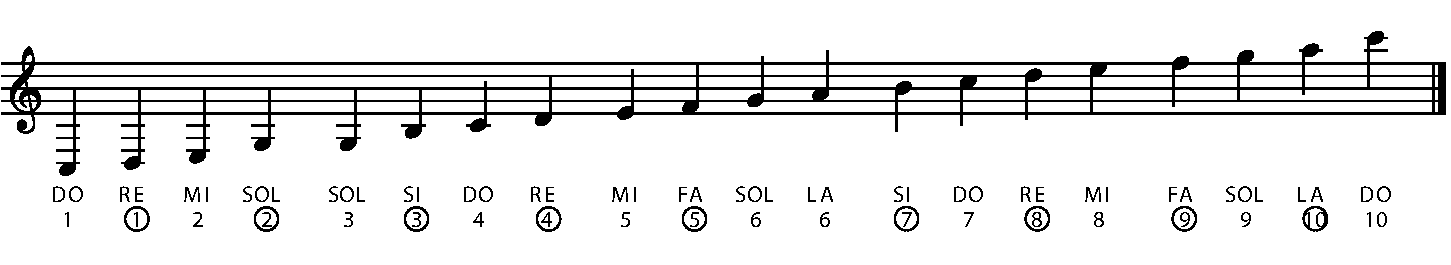
\includegraphics[width=\textwidth]{chapters/SPARTITO ARMONICA.pdf}
\end{center}

Simbologia utilizzata:
\begin{enumerate}
\item[\asp{4}] : foro 4 aspirato
\item['] : Bending di un semitono
\item[''] : Bending di due semitoni
\item[>>] : Passaggio rapido alla nota sucessiva
\item[$\rightarrow$] : Mantenimento lungo della nota
\item[\underline{\asp{4}}] : durata doppia della nota
\item[$\square$] : pausa
\end{enumerate}